\documentclass[10pt,twoside]{book}

\usepackage{graphicx}

\oddsidemargin=-5mm
\evensidemargin=-5mm
\topmargin=-5mm
\textwidth=170mm
\textheight=240mm

\pagestyle{myheadings}

\markboth{\dotfill MeqTree Kernel Design Overview}{\small\tt
LOFAR/doc/MEQ/MeqDesignOverview.tex\em~~$\circ$~$ $Revision$ $~$\circ$~$ $Date$ $\dotfill}

\title{{\sf MeqTree Kernel Design Overview (PSS4)}}

\author{{\sf O.M. Smirnov}}

\date{\vspace{2cm}\small CVS path: \tt LOFAR/doc/MEQ/MeqDesignOverview.tex\\\rm
$ $Revision$ $\\$ $Date$ $}



\begin{document}

\sloppy

\newcommand{\url}[1]{{\tt #1}}

\maketitle
\tableofcontents

% \qq{text} used to quote code (in fixed font)
\newcommand{\qq}[1]{{\tt #1}}

\newcommand{\Request}{{\tt Request}}
\newcommand{\RequestId}{{\tt RequestId}}
\newcommand{\Result}{{\tt Result}}
\newcommand{\VellSet}{{\tt VellSet}}
\newcommand{\Cells}{{\tt Cells}}
\newcommand{\Vells}{{\tt Vells}}
\newcommand{\Domain}{{\tt Domain}}
\newcommand{\Node}{{\tt Node}}
\newcommand{\Parm}{{\tt Parm}}
\newcommand{\Polc}{{\tt Polc}}
\newcommand{\RES}[1]{{\tt RES\_#1}}

\chapter{The Fundamentals}

  The purpose of this document is to provide an overview of the MeqTree kernel
  and related interfaces. The following subjects will be covered:

  \begin{itemize}

  \item Basic terms and concepts.

  \item System components.

  \item Data structures employed in the MeqTree kernel.

  \item Standard node state \& functionality.

  \item Interaction between nodes, and how it is affected by state.

  \item Interaction with Glish (and in the future, other scripting languages).

  \item Examples of some standard and application-specific nodes.

  \end{itemize}

  The intended audience for this document is:

  \begin{description}

  \item[The Tree Designer,] since a thorough understanding of how nodes interact
  is critical in construction of complex and efficient trees.

  \item[The Node Developer] needing to implement specialized node classes.

  \end{description}


\section{Trees}

  The MeqTree kernel provides a C++ implementation of the MeqTree concept. A {\bf
  MeqTree} (or simply ``tree'') is a collection of interconnected {\bf MeqNodes}
  (or simply ``nodes''). Nodes have a directed parent--child relationship; a
  parent may have any number of children, and a child can have multiple parents.
  Cycles are forbidden. Technically, this makes the MeqTree a {\em directed
  acyclic graph}, but the term ``tree'' is retained for historical and
  aesthetical reasons.

  We will often use directional terms when discussing trees, {\bf up} is from
  parent to child, and {\bf down} is from child to parent.

  In broad terms, the life of a node generally consists of receiving {\bf
  requests} from its parent(s), passing them on to its children, receiving {\bf
  results} in response, performing some calculation on the child results, and
  returning the result of that its parent. Thus, requests generally originate
  somewhere down the tree and propagate up, while results germinate at the top
  and percolate down. 

\section{Nodes}

  Nodes are implemented as C++ objects, subclassed from the abstract
  \qq{Meq::Node} class\footnote{All the MeqTree kernel classes reside in the
  \qq{Meq} namespace; we will omit \qq{Meq::} from names from now on.}. All
  interaction with nodes is done via the \Node\ class interface. Consequently, a
  node has no direct knowledge of the {\em type} of its children. Nodes may be
  connected together in a practically arbitrary manner. Given a rich toolbox of
  elementary node classes, trees representing arbitrary mathematical expressions
  may thus be constructed. 

  All nodes have a {\bf state record} that determines their behaviour. The state
  record is fully accessible from the outside. The initial state record is also
  called the {\bf defrec} (from definition record), and is usually supplied from
  the scripting layer when the node is created.

  Nodes also have a {\bf result cache} that may retain the most recently computed
  result. The cache is intended to save processing time for repeated (or similar
  enough) requests.

\section{Design philosophy}

  These principles are key to understanding the design philosophy behind the
  kernel:

  \begin{description}

  \item[Locality:] all functionality is defined in terms of local parent--child
  request--result interactions. There is no centralized ``control'' as such.

  \item[KISS the nodes and rely on emergent behaviour:] complex behaviour of the
  tree as a whole emerges from primitive request--result interactions at the
  local level. Most node classes are designed to be simple (K.I.S.S.!), with a
  single well-defined purpose. If some sort of specific functionality is
  required, it is almost always preferrable to implement it by building the right
  tree, rather than developing specialized nodes.

  \item[Policy-free:] kernel node classes are largely policy-free. By policy we
  mean any sort of application-specific behaviour or concepts. Policy may only
  emerge at the tree level (by connecting the nodes in a specific way), and/or at
  the scripting level.

  \item[There is more than one way to do it:] (with a nod to Larry Wall and Perl)
  in a lot of cases, the kernel provides several ways of accomplishing the same 
  result. There is not necessarily a single ``right'' way, it all depends on the
  particular application context. This redundancy is by design, as it increases
  the overall adapatability of the system.

  \end{description}

\section{Software components}

  An interface to the kernel is provided via a \qq{MeqServer} object. The
  \qq{MeqServer} maintains a {\bf forest} (a collection of nodes and trees), and
  provides operations such as:

  \begin{itemize}

  \item Create, connect and delete node objects.

  \item Inspect and modify node state records.

  \item Issue requests and return results.

  \item Connect trees to data sources (e.g. Measurement Sets).

  \end{itemize}

  \qq{MeqServer} plugs into the OCTOPUSSY publish/subscribe framework, and
  thorugh it can can transparently support any number of local or remote clients,
  such as Glish sessions.

  All application-dependent logic (``policy'') is meant to reside in the scripting
  layer (Glish, and in the future Python).

\chapter{Data Structures} 

\section{Basic concepts}

  The main priciple driving data structure design in MeqTrees is {\bf
  congruity}: all C++ objects used to {\em pass information} within a tree must
  be mappable without any loss of information to and from data structures on
  the scripting side. Fully {\em private} structures (e.g., private nested
  classes) can exist on the C++ side only.

  Congruity facilitates {\bf transparency}: most of the inner workings of a
  tree are readily accessible from the scripting side. This allows for very
  elaborate monitoring schemes, and is a great debugging aid when something
  goes wrong.

\subsection{Data types}
  
  The choice of atomic data types is limited by the requirement of congruity.
  Currently, the only supported scripting language is Glish, but Python 
  support is expected in the near future. In any case, the kernel  restricts
  itself to common primitives that are supported by all mature scripting
  languages. Thus, kernel data structures are defined in terms of a restricted
  set of ``legal data objects'', specifically:

  \begin{itemize}
  
  \item scalars -- bool, integer, float, double, float or double complex;
  
  \item strings;
  
  \item multidimensional arrays of scalars;
  
  \item lists of legal objects (in Glish this is represented either  via a
  vector of scalars or strings, or via a record with fields indexed by number);

  \item records of legal objects (a.k.a. dictionaries/maps/hashes with a string
  key and a legal object value).

  \end{itemize}

  On the C++ side, data objects are based on the DMI \qq{DataRecord},
  \qq{DataField} and \qq{DataArray} classes. Most data classes are in fact
  derived from \qq{DataRecord}, and are at core a record with some (sometimes
  loosely) predefined structure.

\subsection{HIIDs}

  The \qq{HIID} (hierarchical indentifier) class of the DMI package is used for
  all data-related indentifiers in the kernel, such as record fields, node
  groups, request IDs, etc.
  
  A HIID is essentially a vector of integers called {\em atomic IDs}. Atomic
  IDs have a string representation: for IDs $>=$0 this is simply the integer
  itself in string form, while for IDs $<$0, a global {\em dictionary} (i.e.
  map from strings to numbers) is maintained in the development tree. Another
  way to look at this is that negative IDs represent {\em atomic concepts}, or
  words. Thus, any HIID can be viewed as a mix of words (from a fixed though
  rather large vocabulary!) and numbers.

  The string form of a HIID consists of atomic IDs, separated by periods. For
  example, \qq{"Request.ID.1"} is the string form of $(-1210,-1087,1)$. Note
  that the string form is {\bf not} case-sensitive, so \qq{"request.id.1"}
  corresponds to the same HIID. An alternative string representation, employing
  underscore (\qq{"\_"}) as the separator, is used for Glish record fields,
  e.g., \qq{rec.request\_id\_1}. 

  The reason we use such HIIDs instead of plain strings is efficiency on the
  C++ side -- many data storage classes engage in parsing or building up HIIDs,
  and vectors of integers are much easier to manipulate than strings. Note that
  the symbol-to-ID mapping is also available as C++ header files containing
  \qq{const} declarations for atomic IDs. These may be used as, e.g.:

  \begin{verbatim}
  const HIID MyFieldName = AidRequest | AidId | 1;
  \end{verbatim}
  
  is a convenient and visually obvious way to define a constant HIID
  corresponding to \qq{"Request.ID.1"}. The compiler turns this declaration
  into a constant vector of integers.

  HIIDs are covered in more detail in the documentation for DMI. Here we'll
  only dwell on their Glish form. There's two forms in which HIIDs appear in
  Glish:
  
  \begin{itemize}
  
  \item As record field names, e.g., \qq{rec.request\_id}. The implication of
  this is that in order to be recognized by the kernel, all record field names
  must be built up from a fixed vocabulary (which may be extended by the
  C++ developer as new classes are added).

  \item As values. In Glish, a HIID value is just a string containing the
  HIID's symbolic form, tagged by the \qq{::is\_dmi\_hiid} attribute. The
  \qq{hiid()} function (in \qq{dmitypes.g}) is a convenient way to create HIID
  values. For example:

  \begin{verbatim}
  my_id := hiid('Request.ID.1');
  my_id := hiid('request','id',1);
  \end{verbatim}
  
  will both create the same HIID. 
  
  Note the crucial difference between strings and HIID values. Compare the two
  Glish records:

  \begin{verbatim}
  rec1 := [ a = 'a.b.c.1' ];
  rec2 := [ a = hiid('a.b.c',1) ];
  \end{verbatim}
  
  While they may appear to be practically identical on the Glish side of things
  -- both records contain the string field \qq{a}, except \qq{rec2.a} has an
  extra attribute tag -- when passed to the C++ kernel, \qq{rec1.a} is
  converted to an \qq{std::string} object, while \qq{rec2.a} is converted to a
  \qq{HIID} object.
  
  \end{itemize}

  In this document, we will use both forms interchangably depending on context,
  with the understanding that, e.g., \qq{request\_id\_1} and \qq{"Request.ID.1"}
  both refer to the thing as far as the kernel is concerend.

\subsection{Naming conventions}

  \begin{itemize}

  \item In C++, standard data structures \& nodes reside in \qq{namespace Meq}.
    In Glish, corresponding object constructor functions are placed into the
    {\tt meq} ``namespace'' (actually just a record), and names are
    all-lowercase. The DMI dynamic type system uses a {\tt Meq} prefix for the
    namespace. Thus, the \qq{Meq::\Request} class in C++ is registered as a
    ``\qq{MeqRequest}'' in the DMI type system, and  has a \qq{meq.request()}
    counterpart in Glish.

  \item Even though the languages we use are case-sensitive, HIIDs aren't. A
    good reason to avoid relying character case to distinguish identifiers is
    that different languages and contexts have different capitalization
    conventions -- compare, e.g., \qq{Meq::Request} in C++, as opposed to
    \qq{meq.request} in Glish. Thus we should always avoid assigning
    case-sensitive names to different entities.

  \end{itemize}

\subsection{Glish \qq{meq} objects: meqtypes.g}

  With a couple of exceptions, Meq objects are represented by Glish records of
  a [mostly] predefined layout. The Glish/C++ conversion layer uses a few
  ``magic'' attributes to distinguish these objects from ordinary records, so
  it is able to map them to specialized Meq C++ classes rather than generic
  \qq{DataRecord}s. 

  Specifically, the \qq{::dmi\_actual\_type} attribute is set to a string which
  gives the DMI object type. Thus, it is possible to construct a record in
  Glish, tag it with \qq{::dmi\_actual\_type}, pass it thorugh the Glish/C++
  layer, and have it auto-magically converted to an C++ object of the
  appropriate class. The only requirement is that the record contain the
  correct set of fields, which are mapped to class attributes (data members) in
  C++. The file \qq{meq/meqtypes.g} defines  some Glish ``constructor''
  functions which create properly formed records\footnote{Note that some Meq
  classes may have Glish counterparts but no Glish constructors. At time of
  writing, these include \Vells, \VellSet{}s, and \Result{}s. The reason for
  this is simply lack of necessity, since objects of these classes always
  originate on the C++ side rather than Glish. In the future, constructors for
  these classes may be added to Glish as required.}:

  \begin{description}
  
  \item[\qq{meq.domain()}] creates a Domain object (record).

  \item[\qq{meq.cells()}] creates a Cells object (record).

  \item[\qq{meq.requestid()}] creates a request ID from individual components
  (e.g., domain ID, config ID, iteration ID). A request ID is really just a
  \qq{HIID}.

  \item[\qq{meq.request()}] creates a Request object (record).
  
  \item[\qq{meq.polc()}] creates a Polc object (record).
  
  \end{description}
  
  In general, all data objects on the C++ side have counterparts on the Glish
  side. Within this document, we will usually describe data objects in terms of
  their Glish equivalents -- records and record fields -- with the implied
  understanding that there is a 1:1 mapping from that to C++ classes and data
  members.

\subsection{Glish lists}

  Glish does not have a native ``list'' (a.k.a. ``sequence'') construct.
  Instead, lists are emulated in one of two ways:

  \begin{itemize}

  \item If all list elements are all of the same {\em scalar} type,
  then the list is emulated by a vector.
  
  \item If the list elements are of a non-scalar type, or the type is not
  homogenous, then the list is emulated by a record.\footnote{When mapping lists created
  in the kernel to Glish records, the conversion layer assigns field names of
  the form \qq{"\#1"}, \qq{"\#2"}, etc.}
  \end{itemize}

  Since Glish records support numeric subscripts, both types of lists can be
  accessed via the same syntax -- \qq{len(list)} returns the number of
  elements, \qq{list[$n$]} accesses element $n$. Note though that if a list
  contains only one element, it should still be accessed as \qq{list[1]} rather
  than \qq{list} (the latter syntax will actually do the right thing given a
  vector, but not a record, hence it should be avoided for consistency's sake.)

  We will use the term {\em list} from now on to refer to both types of Glish
  structures, as it should usually be clear from context which type is actually
  employed.


\subsection{1-based and 0-based indexing}
  \label{sec:indexconv}

  Glish array indices are 1-based, while C++ indices are 0-based. This,
  unfortunately, has always lead to all sorts of confusion, since indices pop
  up on both sides of the Glish/C++ barrier, and sometimes even need to be
  passed back and forth. As our experience with AIPS++ has shown, keeping track
  of index conversion on an individual basis is completely impractical.

  {\bf The Glish/C++ conversion layer attempts to address this issue by
  providing {\em automatic conversion} of indices. If a record field's name
  ends in \qq{\_index} (on the C++ side this corresponds to a field HIID ending
  in the atomic ID \qq{"Index"}), and the field contains a single integer or a
  list of integers, then the field is assumed to contain indices, and
  conversion between 0- and 1-base is automatically performed.}

  Thus, the Glish record \qq{[foo=1,foo\_index=1,bar\_index=[2,3]]} will be
  converted to \qq{[Foo=1,Foo.Index=0,Bar.Index=[1,2]]} on the C++ side (and
  vice versa), while \qq{[foo\_index=1.0]} or \qq{[foo\_index=[a=1,b=2]]} will
  not undergo any conversion (since the \qq{\_index} field contains a
  \qq{double} value in one case, and a subrecord in the other case).

  Automatic conversion, of course, introduces its own potential for confusion
  if forgotten about. This is why you simply shouldn't forget about it. As a
  visual aid, the paragraph above is highlighted in bold.

\section{MeqRequest and related data objects}

  A \Request\ is a {\em job description} containing a number of commands that a
  node executes in order to produce a \Result. A \Request\ is implemented as a
  record with a semi-fixed structure; commands correspond to specific field 
  names, while the value of each field usually carries the command arguments.
  
  Operationally, the critically important command is \qq{cells}: this tells the
  node to evaluate itself over a given grid in the frequency--time domain. In
  fact, most other commands are mere housekeeping, while \qq{cells} represents
  the brunt of the workload. For this reason, the \qq{cells} command gets
  special treatment: it is placed at the top level of the request record (along
  with a few related flags), and all nodes are obliged to process it. All other
  commands are kept inside a {\bf rider} sub-record, and are subject to a {\em
  node selection} mechanism that allows commands to be directed to all nodes,
  individual nodes, or groups of nodes (this is described in further detail in
  section~\ref{CSR}).

  Each \Request\ is assigned unique request ID ({\bf rqid}, pronounced
  ``arr-cue-d''). This is a \qq{HIID} describing various properties of the
  request. Request generators are expected to follow a certain {\em contract},
  and assign rqids in a consistent way. This is covered in detail in
  section~\ref{sec:rqid}.

  On the C++ side, a \Request\ is derived from \qq{DataRecord}. It can contain
  the following fields (of which only request\_id is obligatory).
  \vspace{1em}

  \noindent\begin{tabular}{l|l|p{.7\textwidth}}
  \hline
  {\scriptsize\sf field name } & {\scriptsize\sf type} & {\scriptsize\sf description}\\
  \hline
  \qq{request\_id} & \qq{HIID} & the request ID\\
  \qq{cells}       & \qq{Cells} & {\em [optional]}~~a \Cells\ object (see below)\\
  \qq{calc\_deriv} & \qq{int} & {\em [optional]}~~compute perturbed values (0, 1 or 2).
                      Default is 0.\\
  \qq{next\_request} & n/a & {\em [optional]}~~a hint of what the next request is going to be.
                      This influences caching decisions and speculative
                      execution (section~\ref{sec:nextreq}). {\em This is not
                      currently implemented.}\\
  \qq{rider}       & \qq{record} & {\em [optional]}~~rider subrecord containing additional commands.
  \\\hline
  \end{tabular}\vspace{1em}
  
\subsection{Constructing Requests}
  
  In Glish, a \Request\ record can be created by calling the following
  function:

  \begin{verbatim}
  meq.request := function (cells=F,request_id=F,calc_deriv=0)
  \end{verbatim}
  
  You can subsequently add commands to the record using \qq{meq.add\_command()}
  and \qq{meq.add\_state()}. This is also described in section~\ref{sec:CSR}.
  
\subsection{Domains and Cells}

  The \qq{Domain} class represents a rectangular domain in frequency--time
  space. The \qq{Cells} class represents a gridding of that domain. This is
  illustrated by Figure~\ref{fig:cells}.
  
  \begin{figure}
  \begin{centering}
  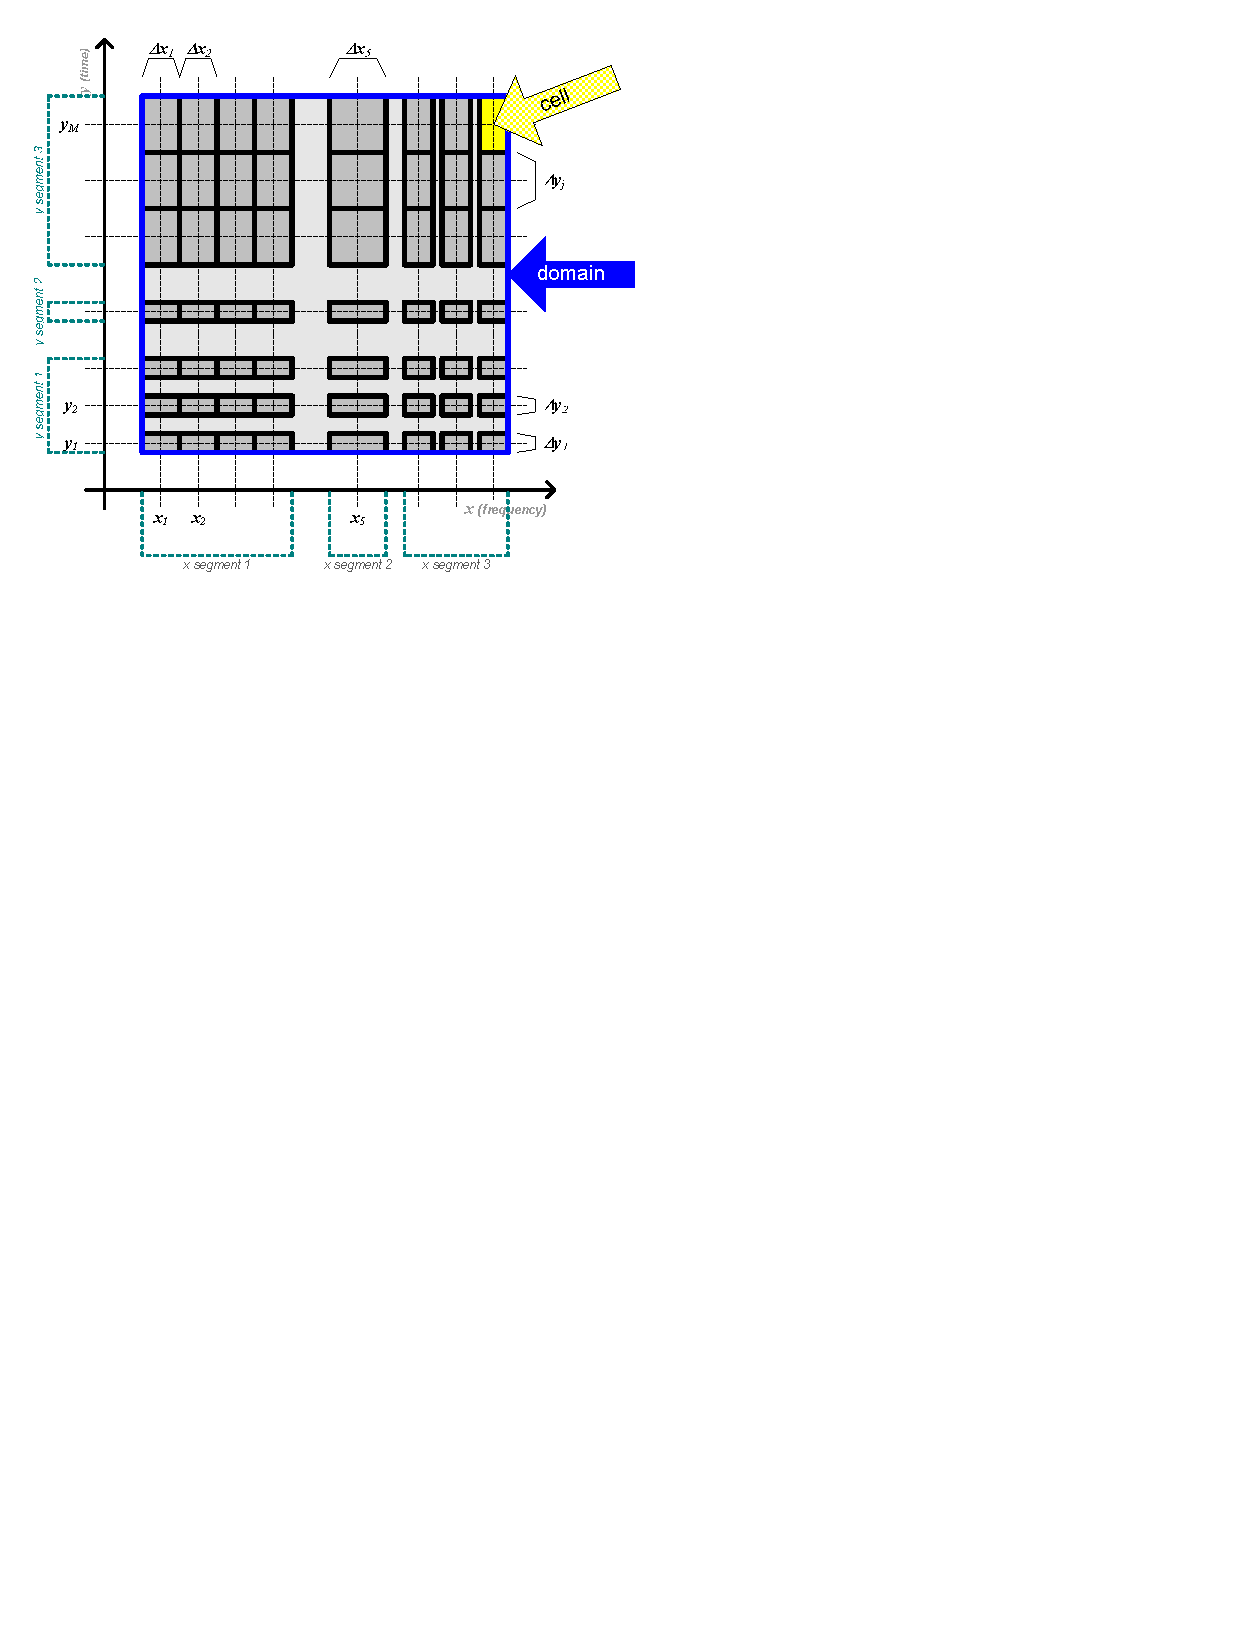
\includegraphics[width=.5\textwidth]{Figures/Cells.eps}\\
  \end{centering}
  \caption{\label{fig:cells}Layout of a Cells object and the envelope Domain}
  \end{figure}
  
  On the C++ side, both classes are derived from \qq{DataRecord}. A \Domain\ 
  record corresponding to $[f_{st},f_{end}]\times[t_{st},t_{end}]$ has the following structure:
  
  \qq{[ freq = [ $f_{st},f_{end}$ ], time = [ $t_{st},t_{end}$ ] ]}
  
  where $f_{st},f_{end},t_{st},t_{end}$ are \qq{double} values giving the domain
  boundaries.

  Note that the specific concepts of {\em frequency} and {\em time} are
  meaningful to only a handful of nodes. The majority of nodes simply deal in
  functions defined over abstract 2D space (to be precise, with 
  $\mathcal{R}^2\rightarrow\mathcal{R}$ or
  $\mathcal{R}^2\rightarrow\mathcal{C}$ functions), without associating any
  semantics with the dimensions. For this reason, the bulk of kernel code is
  careful to abstract itself from the \qq{freq} and \qq{time} names whereever
  possible, treating domain components only as ``first axis'' and ``second
  axis''. The Glish syntax of selecting record fields by number is handy here:
  if \qq{dom} is a domain record, then \qq{dom[1]} and \qq{dom[2]} refer to the
  axis subrecords in a name-independent way.

  The \Cells\ record is structured in the same spirit:
  
  {\tt\begin{tabular}{lrl@{}l}
  [ &domain~&     = [ {\em envelope domain record} ],\\
    &grid~&       = [ freq = [$f_1,...,f_N$],~&~time = [$t_1,...,t_M$] ],\\
    &cell\_size~& = [ freq = [$\Delta f_1,...,\Delta f_N$],~&~time = 
                              [$\Delta t_1,...,\Delta t_M$] ],\\
    &segments&\multicolumn{2}{l}{=~[ freq =
    [start\_index=[$i'_1,...,i'_n$],end\_index=[$i''_1,...,i''_n$]],}\\
              &&\multicolumn{2}{l}{~~~~time =
              [start\_index=[$j'_1,...,j'_m$],end\_index=[$j''_1,...,j''_m$]] ] ]}\\
  \\ 
  \end{tabular}}
  
  This represents an $N\times M$ gridding of the given domain. The $[f_i]$ and
  $[t_j]$ vectors give the cell centers, while $[\Delta f_i]$ and $[\Delta
  t_j]$ give the cell sizes. 
  
  The \qq{segments} sub-record contains information on the {\bf regular
  segments} of the grid.\footnote{Some calculations, such as the DFT, can be
  significantly optimized over regular grids.} A regular segment is a part of
  the grid over which the stepping between cell centers, as well as the cell
  size, remains constant. The \qq{start\_index} and \qq{end\_index} vectors
  contain the starting ($i',j'$) and ending ($i'',j''$)
  indices\footnote{1-based in Glish, 0-based in C++, see
  section~\ref{sec:indexconv}.} of each regular segment.
  By definition, given $n$ segments and $N$ grid points, $i'_{k}= i''_{k-1}+1$,
  $i'_1=1$, $i''_n=N.$

  In the simplest case, the entire $N\times M$ grid is regular, in which case the
  \qq{segments} subrecord looks like this:
 
  {\tt\begin{tabular}{ll}
  [&freq=[start\_index=[1],end\_index=[$N$]],\\
  &time=[start\_index=[1],end\_index=[$M$]]~~~~]\\
  \end{tabular}}
  
  The other extreme, of course, is the completely irregular grid. This is
  represented by \qq{segments} of the form:

  {\tt\begin{tabular}{ll}
  [&freq=[start\_index=[1,2,$...N$],end\_index=[1,2,$...N$]],\\
  &time=[start\_index=[1,2,$...M$],end\_index=[1,2,$...M$]]~~~~]
  \end{tabular}}
  
  Figure~\ref{fig:cells} shows an $8\times7$ grid with three regular segments
  along each axis. This would correspond to the following \qq{segments}
  sub-record:

  {\tt\begin{tabular}{ll}
  [&freq=[start\_index=[1,5,6],end\_index=[4,6,8]],\\
   &time=[start\_index=[1,4,5],end\_index=[3,5,7]] ]
  \end{tabular}}
  
  Note that \qq{segments} information is merely an optimization facility, and
  can be safely ignored most of the time. The user need not know anything about
  it, since \Cells\ constructors compute \qq{segments} automatically; most
  application code doesn't care either, instead working directly with the
  \qq{grid} vectors. 

  On a related note, the \Cells\ record is full of redundant information. For
  example, \qq{domain} and \qq{segments} can be completely derived from
  \qq{grid} and \qq{cell\_size}. This has two important implications:
  
  \begin{itemize}
  
  \item To construct a \Cells, you need to provide only the minimum sufficient
  information, while the constructor figures out everything else automatically.

  \item \Cells\ records should be treated as read-only. Directly manipulating 
  any of the values inside can break consistency between the
  grid/domain/segments fields, and lead to all sorts of confusion down
  the line.

  \end{itemize}
  
\subsubsection{Constructing \Domain{}s and \Cells{}}

  The Glish \qq{meq.domain{}} function constructs a record corresponding to
  a \Domain\ object. Its usage is pretty much self-evident:
  
  \begin{verbatim}
    meq.domain := function (startfreq,endfreq,starttime,endtime)
  \end{verbatim}
  
  The \qq{meq.cells()} function is somewhat more elaborate:
  
  \begin{verbatim}
    const meq.cells := function (domain=F,num_freq=F,num_time=F,
                                 freq_grid=[],time_grid=[],
                                 freq_cell_size=[],time_cell_size=[])
  \end{verbatim}

  All of the arguments are optional, allowing different ways of specifying 
  a \Cells. For example,
  
  \qq{~~cells := meq.cells(meq.domain(0,1,0,1),2,2);}
  
  creates a regular $2\times 2$ grid for the domain $[0,1]\times[0,1]$: cell
  centers at (0.25,0.75), cell sizes of (0.5,0.5). The same \Cells\ can be
  alternatively specified as:
  
  \qq{~~cells := meq.cells(freq\_grid=[0.25,0.75],time\_grid=[0.25,0.75]);}
  
  letting the constructor derive the domain \& cell size automatically. The
  two forms can even be mixed:
  
  \qq{~~cells := meq.cells(meq.domain(0,0,0,1),freq\_grid=[0.25,0.75],num\_time=2);}
  
  produces the same \Cells\ yet again -- note that the \qq{freq\_grid} 
  values override the \qq{freq} component of the domain.
  
  If not supplied in the function call, the default cell sizes are computed to
  perfectly tile the specified domain. The \qq{freq\_} and
  \qq{time\_cell\_size} arguments allow you to supply explicit cell sizes.
  These may be scalars -- implying the same size for all cells along that axis
  -- or vectors. In the latter case, the size of the vector must match
  the corresponding \qq{$x$\_grid} or \qq{num\_$x$} argument.

\section{Fail-records}

  Run-time errors during execution are reported via special structures called
  fail-records. Because fail-records can appear within different data
  structures (see below), they deserve to be documented separately. A
  fail-record has the following layout: \vspace{1em}

  \noindent\begin{tabular}{l|l|p{.7\textwidth}}
  \hline
  {\scriptsize\sf field name } & {\scriptsize\sf type} & {\scriptsize\sf description}\\
  \hline
  \qq{message} & \qq{string} & a description of the error.\\
  \qq{node\_name} & \qq{string} & {\em [optional]}~~name of originating node, if any.\\
  \qq{node\_class} & \qq{string} & {\em [optional]}~~classname of originating node, if any.\\
  \qq{origin} & \qq{string} & origin: usually just the source file name.\\
  \qq{origin\_line} & \qq{int} & origin location: usually just the source line number.\\
  \hline
  \end{tabular}\vspace{1em}
  
  Because most errors tend to cascade from lower-level subsystems up to the
  application level, accumulating more specific descriptions along the way,
  fail-records usually come in a list. Lower-level errors then appear up at the
  head of the list, and higher-level errors appear at the tail.
  
  Certain data classes described below (e.g., \qq{Result} and \qq{VellSet})
  support a fail state -- i.e., a form of the data object describing a failure.
  A fail state is represented by a record with a single field named \qq{fail},
  containing a list of fail-records. In fact, all Glish code can follow the
  simple policy that any record with a \qq{fail} field describes an object in
  fail state, that \qq{fail} contains a list of fail records, and that no other
  meaningful fields are to be found in the record.
  
  
  
  
  

\section{MeqResult and related data objects}

  A \Result\ contains the result of a \Request's execution. A \Result\ is also
  a record (derived from \qq{DataRecord} on the C++ side). Theoretically, this
  record is completely free-form, with its contents dependant on the commands
  in the original \Request\ (and in some cases even on node type -- e.g., a
  \qq{Solver}'s result will contain solution metrics). If, however, the
  original \Request\ contains a \qq{cells} command -- asking the node to
  evaluate itself over the given \Cells\ -- and the command is executed
  successfully, then the returned \Result\ has a well-defined structure:
  \vspace{1em}

  \noindent\begin{tabular}{l|l|p{.7\textwidth}}
  \hline
  {\scriptsize\sf field name } & {\scriptsize\sf type} & {\scriptsize\sf description}\\
  \hline
  \qq{cells}  & \Cells & the \Cells\ of the result (not necessarily matching the request cells
  -- see discussion below)\\
  \qq{values} & \VellSet[] & list of result values\\
  \qq{integrated} & \qq{bool} & flag indicating if the values are integrations or
                    samplings (default is false, implying samplings)\\
  \hline
  \end{tabular}\vspace{1em}
  
  A \Result\ can represent both a sampling of some function at the cell
  centers, or an integration over each cell. The \qq{integrated} flag is used
  to indicate this, if missing, \qq{false} (i.e. a sampling) is assumed. Leaf
  nodes set this flag according to the type of value they return (for example,
  a \qq{Spigot} reading visibilities from a data set returns integrations; a
  \qq{Parm} representing gain returns samplings). Non-leaf nodes should take
  care to pass this flag from child to parent properly. This flag is also taken
  into account when performing resampling of results
  (section~\ref{sec:resampling}).
  
\subsection{Multiple values}
  
  Note that the \qq{values} field is defined as a {\em list} of \VellSet{}s. In
  Glish, a list is implemented as a record, using the \qq{rec[1]}, \qq{rec[2]},
  etc. syntax to access fields by number. Even if there is only one \VellSet\
  in the list, you still have to access it as \qq{result.values[1]}.

  The point of defining a \Result\ as a set of \VellSet{} values (as opposed to
  a single value) is to allow multiple return values for a single \Cells\
  (a.k.a. ``multiple planes''). For example, a \qq{Spigot} may return four
  values at a time (for the four correlations). Function nodes expect all child
  \Result{}s to either have the same number of planes, and will apply the
  function to each set of planes (cross-slice) independently; however, some
  children may have only one plane, in which case it is re-used in each
  cross-slice.

  The \qq{Selector} and \qq{Composer} nodes can be used to decompose and
  assemble \Result{}s.

\subsection{Fail-results}

  Run-time errors arising during a \Request{}'s execution produce a special
  kind of \Result\ called the fail-result, which describes the error. A
  fail-result record contains only one field called \qq{fail}, containing
  a {\em list} of fail records.
  
  record does not have a \qq{cells} field, and its \qq{values}
  field contains one or more fail-\VellSet{}s (see below). 

\subsection{VellSet}

  A \VellSet\ record describes a $\mathcal{R}^2\rightarrow\mathcal{R}$ or
  $\mathcal{R}^2\rightarrow\mathcal{C}$ function over some \Cells\ (i.e. domain
  \& gridding). It contains the function value (as an object called a \Vells),
  plus optional {\em perturbed values} -- the values of the function given
  small perturbation in parameters (indentified by their {\bf spids}, for
  solvable parameter IDs) -- which then can be used to estimate derivatives.

  On the C++ side, \VellSet\ is derived from \qq{DataRecord}. The \VellSet\
  record has three forms: regular, empty and fail.
  
  \subsubsection{Regular VellSets}
  
  The regular form of a VellSet contains the following fields:

  \vspace{1em}
  
  \noindent\begin{tabular}{l|l|p{.7\textwidth}}
  \hline
  \qq{value}  &  the \Vells\ corresponding to the function value.\\\hline
  \multicolumn{2}{l}{~~~~\em optional, only appears if \qq{calc\_deriv>0} was specified in
  the original \Request:}\\
  \qq{spids}  &  a list of integer spids identifying the parameters
                for which perturbed values are provided\\
  \qq{perturbations}  & a list of parameter 
                        perturbations (must be same length as \qq{spids})\\
  \qq{perturbed\_value} & perturbed values: a list of \Vells\ (must
                      be the same length as \qq{spids})\\\hline
  \multicolumn{2}{l}{~~~~\em optional, only appears if \qq{calc\_deriv>1} was specified 
  in the original \Request:}\\
  \qq{perturbations\_1}  & second set of parameter 
                        perturbations (same length as \qq{spids})\\
  \qq{perturbed\_value\_1} & second set of perturbed values (same length as \qq{spids})\\
  \hline
  \end{tabular}\vspace{1em}
  
  \subsubsection{Empty VellSets}

  An empty \VellSet\ is just an empty record, corresponding to a
  default-constructed (empty) object in C++. While empty \VellSet{}s shouldn't
  be present in well-formed results, they can still appear in node state
  records and other structures, thus Glish code should be prepared to deal with
  them.
  
  \subsubsection{Fail-VellSets}

  A fail-VellSets is used to indicate a run-time error or other failure. The
  corresponding record has only one field named \qq{fail}, containing a list of
  fail-records.

  \noindent\begin{tabular}{lp{.8\textwidth}}
  \end{tabular}
                    
  The \qq{value} and \qq{fail} fields are mutually exclusive. A \VellSet\ with
  neither is an empty (uninitialized). A \VellSet\ with a \qq{fail} in it is
  called a fail-\VellSet\ (or simply a fail). The \qq{spids},
  \qq{perturbations} and \qq{perturbed\_value} fields are optional, but either
  none or all three must be present at the same time.
  
  Note also that this layout could be extended in the future to accomodate
  double derivatives and analytic derivatives.

%  \qq{fail}  & a list of one or more fail-records (see below)
%                describing failures that have occurred\\


\subsubsection{MeqVells}

  On the scripting side, a \Vells\ object is simply a scalar or an array. On
  the C++ side, it is also essentially an array, with some run-time type and
  size information. The current implementation supports double and
  double-precision complex types, in either scalar or 2D-array form, but this
  could be extended in the future.

  \Vells\ are covered in some more detail in the description of \qq{Function}
  nodes, below.

\subsection{Multiple values}

  The point of defining a \Result\ as a set of \VellSet{}s is to allow multiple
  return values for a single \Cells\ (a.k.a. "multiple planes"). For example, a
  \qq{Spigot} may return four values at a time (for the four correlations).
  Function nodes expect all child \Result{}s to either have the same number of
  planes, and will apply the function to each set of planes (cross-slice)
  independently; however, some children may have only one plane, in which case
  it is re-used in each cross-slice.

  The \qq{Selector} and \qq{Composer} nodes can be used to decompose and
  assemble \Result{}s.

\subsection{Fail propagation}

  Note that a set may contain a mix of failed and normal \VellSet{}s. Failed
  values should propagate down the tree in an orderly fashion. Normally, a
  fail-value from one of its children produces a fail at the same position in
  the output \Result\ (the contents of the fail -- origin \& description -- are
  preserved.)

  For example, if a \qq{Spigot} node is configured to return four correlations,
  and the data source only has XX and YY, then XY/YXs will be represented by
  fails. These fails would propagate all the way down the XY/YX trees, to a
  \qq{Sink} node, which can handle them benignly (by not writing XY/YX data,
  for example).

\chapter{MeqNode}

  The abstract base class \qq{Meq::Node} implements the basic node behaviour:

  \begin{itemize}

  \item A node may have a number of child nodes. Generally, a node has no
    knowledge of the types of its children. Subclasses may assign formal child
    labels (akin to argument names) to specify semantics, or may leave their
    children unlabeled. Child labels are assigned via the constructor of the
    subclass.

  \item To nail down directional terms: root nodes and parents are at the {\em
    bottom}, children and leaves are at the top. 

  \item Each node is assigned a unique index (integer$>$0) and an optional name. A
    MeqForest object acts as a repository of nodes, and maintains a map between
    names, indices and node objects.

  \item \Node\ has an \qq{execute()} method, taking a \Request\ parameter,
    and returning a \Result. Normally, a node is expected to call execute()
    with the same \Request\ on its children, and form its result based on the
    results of its children. Thus, requests propagate up the tree, and results
    percolate down the tree.
    
A node also has no direct knowledge of its parents, and is only allowed to
infer things from the requests that it receives.


\begin{verbatim}
    virtual int execute (Result::Ref &result,const Request &request);
\end{verbatim}

    \Result{}s are returned by attaching them to the CountedRef. The return code
    of \qq{execute()} is significant; see details below.

  \end{itemize}

\section{Initialization and state}
  
  A node's full {\em state} should be mapped to a {\em state record}. State may
  be requested via \qq{getState()} and changed via \qq{setState()}. Note that
  the argument to \qq{setState()} does not have to be a complete new state
  record; instead, it should contains only those fields that actually need to
  be changed. 

  When a node is constructed, it is passed an {\em init-record} (via the
  \qq{init()} method), which is essentially a complete initial state record.
  This is the way that all run-time arguments to a node are specified! Later 
  in a node's lifetime, the \qq{setState()} method may the be called to
  reconfigure  it. Note that a node class is not obliged to be reconfigurable
  in every single aspect, but it's good design to make it so as much as
  possible. If some of the node state may only be set once via \qq{init()} and
  not changed later on via \qq{setState()} -- call this {\em static\/} state --
  it should be clearly documented as such. The assumed default is {\em
  dynamic\/} state, i.e., state that is freely reconfigurable via
  \qq{setState()}.

  The following methods are responsible for initializing and changing state:

\begin{verbatim}
  // public: Initializes node with init record
  //         Note that Ref::Xfer implies that ref to record will be taken over
virtual void init (DataRecord::Ref::Xfer &initrec);

  // public: Changes dynamic node state (note: non-virtual)
  //         Node can attach to/take over record contents as needed.
void setState (DataRecord &rec);

  // protected: Checks init record for missing fields, fills in defaults where needed
  //            (called from Node::init())
virtual void checkInitState (DataRecord &rec);

  // protected: Implementation for setting or changing internal dynamic state 
  //            (called from Node::setState())
  //            Node can attach to record contents as needed. If initializing,
  //            then record is the state record and should not be changed. If
  //            not initializing, node can take over contents as well.
virtual void setStateImpl (DataRecord &rec,bool initializing);
\end{verbatim}

\subsection{init()}

  The base \qq{Node::init()} does the following:

  \begin{enumerate}
  
  \item Takes over the init record,  sets it as the state record, ensures a
    private \& writable copy.
    
  \item Adds the node's classname (\qq{rec.class}) to the state record if not
    already present. If present, checks that the name actually matches the node
    class.

  \item Calls the virtual \qq{checkInitState()} method with the state record,
    to ensure that it's complete, and that any missing defaults are filled in.

  \item Calls \qq{setStateImpl(staterec,true)} to set up internal state from
    the state record (the \qq{true} argument indicates that the node is being
    initialized with the state record.)

  \item Looks at \qq{rec.children} to set up child nodes. Children may be
    specified via a either a list or a record, containing any mix of the
    following:

    \begin{itemize}
      \item integer node indices referring to existing nodes.

      \item string node names, referring to existing or yet-to-be-created
        nodes. In the latter case, \qq{Node::resolveChildren()} must be called
        later on; this will recursively resolve all children not found at
        \qq{init()} time.

      \item init-records, to recursively create child nodes on-the-fly (each of
        these records must have a field named \qq{class}, containing the child
        node classname).

    \end{itemize}

    If a list is specified, then the children are simply attached in the given
    order. If a record is specified, then the field names must match the child
    labels set up by the subclass (if no labels are set up, the record is
    processed just like a list, with no specific order ensured). The record
    form allows for a more formal child specification in the case where
    children are semantically different.
    
  \item Any errors will result in an exception being thrown at the caller. A
    node object that fails \qq{init()} is under no obligation to be usable; the
    only method that's not allowed to fail is the destructor.

  \end{enumerate}

  Derived classes need to reimplement \qq{init()} only if they have additional
  static state of their own. A derived \qq{init()} should do the following:

  \begin{enumerate}
  
  \item Call the parent class's \qq{init()} with the initrec. This should
    ultimately call \qq{Node::init()}, thus setting up the state record  and
    calling \qq{setStateImpl()} to set up dynamic state.

  \item Set up static state, as defined at the child class level, in accordance
    with the state record.

  \item Throw exceptions on any error. 

  \end{enumerate}
  
  Note the virtual \qq{checkInitState()} method is called from
  \qq{Node::init()}. This is meant to check the init record for required
  fields. The \qq{requiresInitField(record,field)} macro/inline (defined in
  \qq{Node}) is handy for this; it will throw a standard exception if the
  specified field is missing. 
  
  The base \qq{Node::checkInitState()} only fills in a default for \qq{.name}
  (empty). A derived \qq{checkInitState()} should call the parent version, then
  check for additional defaults and required fields as defined by the child
  class.
  
  Note that child classes can also ignore \qq{checkInitState()}, and instead use
  the \qq{initializing} parameter of \qq{setStateImpl()} to determine when
  the node is being initialized, and check for missing fields and/or fill in
  defaults as apporpriate.

\subsection{setState() and setStateImpl()}

  The non-virtual \qq{setState()} method defined in \qq{Node} provides the
  public interface for setting state. Basically, it defers parsing the record
  to \qq{setStateImpl()}, while providing a transaction mechanism of sorts:

\begin{enumerate}

  \item Calls \qq{setStateImpl(rec,false)} to process the record. The
    \qq{false} value indicates that state is being modified rather than
    [re]initialized. (Note that if the supplied record happens to be the node
    state record itself, \qq{true} will be passed in instead.)

  \item Catches \qq{Node::FailWithoutCleanup} exceptions and rethrows them at
    the caller with no additional action.

  \item Catches all other execeptions, and does a cleanup before rethrowing
    them. The cleanup consists of calling \qq{setStateImpl(staterec,true)}, so
    as to reset internal state from the current state record. This is meant to
    roll back from situations where an error midway through \qq{setStateImpl()}
    could cause internal object state to decohere from the state record.

  \item On success, merges the supplied record into the current state record.

\end{enumerate}

  This design ensures that if a \qq{setState()} call fails (i.e., with an
  exception), both the state record and the internal state of the object are
  rolled back to their values prior to the call. (Assuming they were mutually
  consistent to begin with.) In other words, the node object is guaranteed to
  remain usable.

  The virtual \qq{setNodeState()} method is responsible for changing dynamic
  state. It receives two arguments: a \qq{newst} record, and a boolean called
  \qq{initializing}. The latter is \qq{true}, the node is being initialized --
  in this case \qq{newst} is the complete initial state record. If it is
  \qq{false}, \qq{newst} contains only those state fields that are being
  changed. Normally, the method should do the following:

\begin{enumerate}

  \item If the \qq{initializing} is \qq{false}, check the record for
    ``forbidden'' fields, i.e., attempts to modify static state. Throw a
    \qq{FailWithoutCleanup} if any are present. The
    \qq{protectStateField(record,field)}  macro/inline is a convenient way to
    do this.
    
  \item Call the parent \qq{setStateImpl()}.

  \item As an alternative to overriding \qq{checkInitState()}, if
    \qq{initializing} is \qq{true}, check for missing fields and/or fill in
    defaults.

  \item Parse the record and modify internal state relevant to the child class.
    Note that the standard DMI hook method \qq{get()} is very handy for doing
    this operation, combined with the previous one:
    
    \begin{verbatim}
    if( newst[StateField].get(var,initializing) )
      // field is present, react if needed
    else
      // field is missing, react if needed
    \end{verbatim}
    
    The \qq{get()} method employed here does the following: if \qq{StateField}
    is present in the \qq{newst} record, assigns its value to \qq{var}
    (throwing an exception is the types are incompatible) and returns
    \qq{true}. If the field is missing, optionally (only if \qq{initializing}
    is \qq{true}) inits it from the value in \qq{var}, and returns \qq{false}.
    The standard \qq{setStateImpl()} methods make extended use of this
    mechanism.

  \item Throw exceptions on error. A \qq{Node::FailWithoutCleanup} should be
    thrown if and only if no internal state was modified. All other exceptions
    will invoke the ``rollback'' mechanism above. You can rely on
    \qq{DataRecord} (and other DMI classes) to throw an exception when
    datatypes mismatch or something else goes wrong; throw a
    \qq{Node::FailWithCleanup} if you want to indicate some other kind of
    failure.

\end{enumerate}

  The base \qq{Node::setStateImpl()} method is described in detail in a later
  section on basic node state.

\subsection{Unrecognized state fields}

  Note that these implementations of \qq{init()} and \qq{setState()} will
  ignore any unrecognized fields in the init and state record, all the while 
  diligently maintaining and changing them as requested. This allows for a few
  interesting possibilities:

  \begin{itemize}
  
  \item Nodes may be assigned arbitary additional attributes and data,
    meaningless to the node itself, but perhaps useful to the control layer.

  \item Things like the result cache (see below) -- which is stored directly in
    the state record -- may be accessed and changed externally (i.e. from the
    scripting level). This may be useful for debugging and testing.

  \end{itemize}

\section{Node serialization \& persistency}

  In the near future we will need persistent nodes (i.e. being able to
  save/load the nodes to a file or database), and further down the road, the
  possibly the capability to move a node across a network. This implies being
  able to serialize a node.
  
  Serialization is implemented through DMI mechanisms. A \qq{DataRecord} is
  inherently serializable. To serialize a node, the control code will simply
  serialize its state record. To unserialize a node, it will recover the
  record, create a node object (as specified by the \qq{class} field), and call
  \qq{init()} on it. 

  Thus, subclasses of \Node\ should take care to maintain their state record
  appropriately. Each node class should ensure that it is completely
  re-creatable (via \qq{init()}) from a snapshot of its state record at any
  point in time. Basically, this means that a 1-1 mapping should be maintained
  between the state record and internal object state. One possible exception to
  this are internal caches; if these are not maintained in the state record,
  then the worst than can happen from re-creating a node is a cleared cache.
  
\section{Node defrecs}

  Several other functions in \qq{meqtypes.g} help to construct defrecs for
  nodes (see below). \qq{meq.node()} puts together a basic node defrec -- class
  name, node name, optional children specification, optional node group
  list. \qq{meq.parm()} is a specialization for constructing \Parm\ defrecs.


**************************************************************    
  Rqids play a pivotal role in caching behaviour. 
  
  When a node caches a result,
  it also caches the rqid. In the trivial case, if the next request has the
  same ID, the node can immediately return the cached result. In fact the cache
  is somewhat more intelligent. Each cached result also has a {\em dependency
  mask} (or {\bf depmask} for short) that describes {\em what properties of a
  request the result depends on}. Typical dependencies include:

  \begin{itemize} 
  
  \item The request's \Cells\ (envelope domain and grid), obviously enough.
  Example nodes with this dependency: \qq{Parm} (with a non-zero degree
  polynomial), \qq{Time}, \qq{Freq}. 

  \item Only the envelope domain of the \Cells. Example: the \qq{Spigot}, since
  it always returns data at the native resolution of the dataset, ignoring the
  resolution specified in the \Cells.

  \item Updated \qq{Parm} values sent up by a solver.
  
  \item The configuration of a \qq{WSum} node.

  \item Any combination of the above. 

  \end{itemize}
  
  If a node has children, then its result's dependencies are almost always the
  union of the children dependencies, plus (in some cases) additional
  dependencies introduced by the node itself (e.g. the \qq{UVW} node always
  adds a dependency on \Cells). In other words, the depmask of the result is 
  a bitwise-OR of the depmasks of the children's results, OR the node's own
  local depmask. Obviously, the set of dependencies grows as results propagate
  down the tree.

  Given a cached result and its depmask, a node can be somewhat more
  discriminating in choosing when to return a cached result. For example, if
  the depmask indicates that the result depends on \Cells\ only, then all
  further requests with the same \Cells\ can be served from the cache. The same
  applies to other dependencies. In global optimization terms, this means that
  when a tree is re-evaluated for a slightly different request, it recalculates
  only those sub-trees that need it. The problem is how to determine if a
  different request has the same \Cells, without doing a brute-force comparison
  (which can be quite expensive if done at every node). This is where the {\em
  hierarchical} part of request IDs come in.

  An rqid is a \qq{HIID} -- essentially, a string of integer indices. Each
  index corresponds to one bit in the depmask. For example, if the depmask is
  structured as follows:
  
  \begin{tabular}{l|l}
  \hline
  bit 0 & \qq{Parm} values from solver \\
  bit 1 & \qq{WSum} configuration \\
  bit 2 & resolution of \Cells \\ 
  bit 3 & envelope domain of \Cells \\
  \hline\end{tabular}
  
  then the rqid is composed of four indices:
  
  {\tt\em  
  $<$domain index$>$.$<$resolution index$>$.$<$config\_index$>$.$<$value\_index$>$
  }
  
  The decision whether a new request can be served from the cache becomes quite
  simple: just compare all indices of the rqid for which the corresponding
  depmask bit is set, and use the cache only if none of them differ.

  In other words, the components of the rqid describe how a request is
  different from previous requests. The domain index must change whenever a new
  domain is requested, the config index must change whenever a \qq{WSum} is
  reconfigured, the value index must change at each solve iteration, etc.

  Of course, this scheme only works if the depmasks returned by the nodes
  (generally, somewhere up the tree), and the request IDs generated by request
  originators (generally, down the tree) have the same semantics. The
  depmask/rqid correspondence represents a {\em contract} between request
  generators and dependency generators to apply these semantics consistently.
  The \qq{Node} class provides a number of mechanisms for automatically setting
  up consistent semantics throughout the tree, see the discussion on {\em
  symdeps} below.

  Note also that the general scheme implemented at the \qq{Node} level does not
  assume any application-specific semantics at all. The depmask is a treated as
  set of $N$ bits, and the rqid as a corresponding set of $N$ indices.

\subsection{Next\_request and request sequences}

  The concept of a ``request sequence'' has been bandied about a lot (see the
  ``Making Waves'' document, plus various discussions). The reason for this is
  that a node needs some capability of ``looking ahead'' to future requests, in
  order to efficiently utilize cache, and to enable ``rippling'' trees that
  parallelize well.

  In fact, it is sufficient to be able to answer the more limited question:
  given request $X$, what is the next request likely to be? A node doesn't 
  need to know the full request sequence -- only the next step of it. The
  mechanism can be hidden behind a single method called, e.g.,
  \qq{getNextRequestHint()}, implemented at the \Node\ level. This neatly
  factors the issue into two independent ones:

  \begin{itemize}
  
  \item {\em Where does the base \qq{\em Node} class get knowledge of the next
    request?} Obviously, the originator of the \Request\ can have some idea. 
    For example, a \qq{Solver} node would probably know if more iterations over
    the same domain/source are required, or if we're going to the next domain.
    A \qq{Sink} node may know what the next domain is going to be. Etc. It
    seems reasonable to place this information into the \Request\ record
    itself, hence the \qq{next\_request} field.

  \item {\em Given knowledge of the next request, how does that help us in
    caching and parallelization?} Parallelization was the subject of the
    ``Making Waves'' document, while caching issues are discussed below.

  \end{itemize}
  
  The next-request hint is just that, a hint, with no commitment implied. It is
  not necessary at all for correct operation of the system -- even the hint
  itself can even be wrong. The maximum penalty to pay for an incorrect hint is
  recalculation of the tree rooted at the node in question. Efficient
  operation, however, requires that the hint be correct most of the time.

  {\em Hints and sequences are not implemented at the moment; the point of
  the present discussion is to see where this fits into the data structure.}

\chapter{Base Node state}

  The base \qq{Node} class maintains a number of state fields via its
  \qq{setStateImpl()} method. This section describes the state in detail.
  Unless explicitly specified, each state field can be changed dynamically at
  any time. Note that an end user will hardly ever need to change (or even see)
  node state directly; a tree developer, however, will be working with this
  stuff constantly. As will become apparent in this section, a node's internals
  are completely exposed to tweaking and experimentation. The C++ side imposes
  no policy and does very few sanity checks, so it is perfectly possible  to
  thoroughly confuse a node (or an entire tree) through misguided  manipulation
  of its state record from the outside. We assume that it is up to the
  scripting-side tools to shield the end users from ``dangerous'' capabilities.

\section{\qq{class}, \qq{nodeindex}, \qq{children}} 
  
  These fields represent static properties of the node. \qq{setStateImpl()}
  will throw an exception if an attempt is made to change them. \qq{class} is a
  string classname, \qq{nodeindex} is an integer node index, and \qq{children}
  is a list of child node indices (if any).

\section{\qq{name}}
  
  This is just the node name (a string). 
 
\section{\qq{node\_groups}}
  
  A node may be assigned to one or more node groups. The purpose of this is
  described in detail below (see the section on command processing). The
  \qq{node\_groups} field is a list of \qq{HIID} group names. Note that all
  nodes are implicitly members of the \qq{All} group; thus \qq{"All"} is not
  explicitly present in the list.

\section{\qq{auto\_resample}}
  
  This flag specifies if auto-resampling of child results is enabled. See
  detailed discussion later on.

\section{\qq{request\_id}, \qq{cache\_result}, \qq{cache\_result\_code}}
  
  These three fields compose the node result cache. The first field -- a
  \qq{HIID} -- is the ID of the most recent request. The second field is the
  cached \qq{Result} of that request, if any (stored by reference). The third
  field -- an integer -- is the cumulative result code (mainly its the depmask,
  with a few additional flags, described in \qq{execute()} later on) of the
  cached result.

  The node cache may be cleared by assigning a boolean \qq{false} to the
  \qq{cache\_result} field. It is also possible to modify the cache on the fly
  (for example, substituting in another result). This may be a useful feature
  for debugging and experimentation, though if used improperly, it can probably
  confuse the caching and dependency tracking mechanism.  
  
\section{\qq{request}}

  This is a (read-only) reference to the most recently processed \qq{Request}
  object. This field is maintained for information purposes only, \qq{Node}
  fills it whenever it executes a request, but does not use it for anything
  else (so modifying this field will have no effect).

\section{\qq{cache\_policy}}

  This is a placeholder for the caching policy (see discussion below). This is
  not yet implemented -- all current nodes always cache results.

\section{\qq{depend\_mask}, \qq{known\_symdeps}, \qq{active\_symdeps}, 
            \qq{symdep\_masks}, \qq{gen\_symdeps}, \qq{gen\_symdeps\_group}}
              
  These fields are responsible for maintenance of dependency masks. This is a
  somewhat complicated subject covered in a separate section below. Note that
  the default settings for these fields are practically always good enough, but
  they are exposed for purposes of experimentation and debugging.

\chapter{Symdeps and depmasks}

  As discussed in the section on requests above, a {\em depmask} is a bitwise
  mask that describes a result's dependencies on particular properties of the
  request, which are in turn indicated by individual indices of the request ID.
  To enable proper use of the cache, all nodes in the tree should interpret
  these bits and indices in a consistent way -- which is, by necessity,
  application-dependent. Several fields of the node state provide a mechanism
  for setting up these semantics and propagating them throughout trees. 

\section{The local depmask}
  
  The \qq{depend\_mask} field of the state record is the local depmask of the
  node. The local depmask indicates which dependencies a node introduces into
  its result. For most \qq{Function}-derived nodes, this mask is null,
  indicating that the result dependencies are fully determined by child
  dependencies. Leaf nodes, on the other hand, will have a non-null mask.

  The local depmask is automatically ORed into the result code by
  \qq{Node::execute()} (see below). Some nodes will set up the mask at init
  time and never worry about it again. For other nodes, it may change depending
  on node state.

  The depmask is just a set of $N$ bits with no specific semantics associated
  with them. The association between individual bits and specific result
  properties is set up via the mechanism of {\em symbolic dependencies}, or
  {\em symdeps} for short.
  
\section{Symdeps in a nutshell}
  
  A {\em symdep} is a \qq{HIID} (thus, symbolic -- since \qq{HIID}s have a
  symbolic representation) that identifies some application-specific dependency
  of the result. Node classes will typically define some standard symdeps, such
  as these -- used in the standard nodes:

  \begin{description}
  
  \item[``Domain'':] result depends on the requested domain (i.e., the envelope
    domain of the \Cells). Most non-trivial leaf nodes have this symdep.

  \item[``Resolution'':] result depends on the resolution of the \Cells. Most
    nodes with a time and/or frequency dependence have this symdep.
   
  \item[``Parm.Value'':] result depends on parameter values passed up from the
    solver. Solvable \Parm{}s have this symdep.
  
  \end{description}
  
  A node's set of symdeps is generally known to the node class at construction
  time. Then, when a tree is initialized, different symdeps are dynamically
  associated with different bits of the depmask, as described below.
  Essentially, this maps the abstract concepts (the symdeps) onto specific bits
  of the depmasks. In other words, this mechanism is what determines the
  bitmask semantics.

\subsection{Symdep masks}

  Note that certain nodes can be viewed as symdep {\em generators}. These are
  nodes that generate new requests. For example, the \qq{Sink} node generates
  requests with different domains and resolutions, thus we say that \qq{Sink}
  generates the \qq{"Domain"} and \qq{"Resolution"} symdep. The \qq{ModRes} node
  changes the resolution of requests, thus it generates the \qq{"Resolution"}
  symdep. The \qq{Solver} node generates the \qq{"Parm.Value"} symdep.
  
  These nodes are responsible for associating a particular bit of the depmask
  with each symdep that they generate. Typically, they will do this once when a
  tree is initialized. These associations (known as {\em symdep masks}) are
  then recursively sent up the tree, thus becoming known to all child nodes.
  Nodes up the tree can then compute their local depmasks by combining the
  symdep masks of their specific symdeps.

\section{Symdeps: the hairy details}

  This section describes the details of how symdeps and depmasks are set up and
  maintained. Note that all this is maintained in the node state record.

\subsection{Known and active symdeps} 
  
  The {\em known symdeps} of a node are just that, all the symdeps that a node
  class knows about. Typically, this is specified once and for all in the
  node class's constructor, by calling the \qq{setKnownSymDeps()} method.
  
  A subset of the known symdeps -- the {\em active symdeps} set -- determines
  what symdeps currently apply to the node's result. For some node classes,
  this is always the entire known set. Some classes, however, may change their
  active set depending on state. For example, if a \qq{Constant} node is
  configured to provide a constant value as a sampling, then it has no active
  symdeps at all, as the value will be the same for any domain or resolution.
  However, if it is (re)configured to provide the constant as an integration,
  then it begins to depend on resolution -- since the integrated value is the
  product of the sample value and cell size.

  The active symdeps set may be changed by calling the \qq{setActiveSymDeps()}
  method, or by changing the \qq{active\_symdeps} field (a list of \qq{HIID}s)
  of the state record. Whenever this is done, the local depmask is
  automatically recalculated using the known symdep masks, by calling the
  virtual \qq{resetDependMasks()} method.

  The known symdeps may also be changed at any time (though I can hardly see
  why anyone would want to do this), by calling the \qq{setKnownSymDeps()}
  method, or by changing the \qq{known\_symdeps}  field of the state record. 
  
\subsection{Propagating symdep masks}

  A node will automatically keep track of the symdep masks associated with its
  known symdep set. This is done via the rider command facility (see below),
  and implemented via \qq{Node::processCommands()}:

  \begin{itemize}
  
  \item The \qq{Add.Dep.Mask} command contains a map of symdeps to symdep
    masks. (This command usually originates at the symdep generator nodes, see
    ``Generated symdeps'' below). In response to this command, \qq{Node} adds
    all the masks it finds for its known symdeps to its internal map of symdep
    masks. After this, it calls \qq{resetDependMasks()} to recalculate its
    local depmask. 

  \item The \qq{Clear.Dep.Mask} command clears all known symdep masks.
  
  \end{itemize}
  
  One consequence of this design is that each node maintains its own local
  mapping of symdeps to depmasks. While at first glance this may seem redundant
  and even wasteful -- since the mapping would appear to be the same throughout
  a tree -- consider the following points:

  \begin{itemize}
  
  \item When a tree is distributed throughout a cluster, maintaining a single
    ``global'' map becomes difficult (and actually violates the principle of
    locality!) Keeping a copy of the map at each node avoids this problem.

  \item The map is not really global anyway. For example, consider a rippled
    tree with multiple solvers. The solvable parm set of solver 1 and the
    solvable parm set of solver 2 need to be represented by different bits in
    the depmask. Thus, the \qq{"Parm.Value"} symdep of different groups of
    parms will actually be mapped to different depmasks!
    
    Note that node group facility (see processing of rider commands, below)
    provides an elegant mechanism for distributing different symdep masks to
    different node groups.
    
  \item The map is small, and changes very infrequently (if at all -- usually,
    it will be set up only once when a tree is initialized). Thus there is no
    performance cost associated with keeping local copies.

  \end{itemize}
  
  The map of known symdep masks is maintained in the \qq{symdep\_masks} field of
  the node state record. It is possible to change this field on the fly, an
  automatic call to \qq{resetDependMasks()} always results.

\subsection{Generating symdep masks}

  Nodes that generate new requests also need to generate \qq{Add.Dep.Mask}
  commands containing their symdep masks assignments. \qq{Node} provides a
  simple facility for doing this automatically.
  
  A node class can specify its mapping of {\em generated symdeps} to masks
  by calling the \qq{setGenSymDeps()} method at construction time. The standard
  node classes specify some pre-assigned masks by default: bit 0 for
  \qq{"Parm.Value"}, bit 1 for \qq{"Resolution"}, bit 4 for \qq{"Domain"}. This
  allows for simple trees to be put together using just the defaults.
  
  For more elaborate trees -- e.g., rippled trees with multiple solvers --
  different \qq{Solver} nodes need to be assigned different masks for the same
  symdep. This can be done via the \qq{gen\_symdeps} field of the state record.
  This field has to contain a map (e.g. record) of symdeps to depmasks; if
  specified, it overrides any previously set mappings. 
  
  Additionally, a node may be configured to generate symdeps for a particular
  node group only. This useful for, e.g., multiple solvers. By default, the
  \qq{All} group is used, but this can be overridden via the
  \qq{gen\_symdeps\_group} field of the state record.

  Once the generated symdeps are configured, a node needs to be told to send
  them up to its children. This is done by passing it the \qq{Init.Dep.Masks}
  command via a request rider. In responce to this command,
  \qq{Node::processCommands} inserts the appropriate \qq{Add.Dep.Mask} commands
  into the request rider based on the current setting of \qq{gen\_symdeps} and
  \qq{gen\_symdeps\_group}.
  
  Operationally, all this is typically done only once at init time:
  
  \begin{itemize}
  
  \item Request generator nodes are created with an initial state record
    containing their generated symdep assignments (if the default assignments
    need to be overridden).
    
  \item Once all the nodes and trees have been created, a request containing
    two following two commands is given to all the root nodes:
    \qq{Resolve.Children} and \qq{Init.Dep.Masks}. (The first command is
    required to resolve named children).
    
  \item This initial request is propagated up the tree, acquiring symdep masks
    from generator nodes along the way. 
    
  \item All trees are now ready for use.
  
  \end{itemize}

\subsection{Order of state updates}

  Because it is possible to change everything about a node's symdeps and masks
  by modifying the state record, and a state update may contain multiple
  fields, the order in which it is updated becomes important.
  \qq{Node::setStateImpl()} employs the following order:

  \begin{enumerate}
  
  \item Updates the known symdep set from \qq{known\_symdeps}, if specified.
  
  \item If specified, reloads the symdep masks from \qq{symdep\_masks}, and
    calls \qq{resetDependMasks()}.
    
  \item If specified, sets the active symdeps from \qq{active\_symdeps}, and
    calls \qq{resetDependMasks()}.
    
  \item If specified, sets the local depmask from \qq{depend\_mask}.
  
  \end{enumerate}
  
  Basically, this order implies that if the local depmask is explicitly changed
  via \qq{depend\_mask}, the specified value overrides any implict value
  calculated from, e.g., an \qq{active\_symdeps}.
  
\subsection{Specialized node behaviour}  
  
  Note that all these facilities are provided at the basic \qq{Node} level, but
  special node classes are free to ignore them, or make use of only some
  subset. For example, the \qq{Parm} class\footnote{And currently, this is the
  only example.} needs to maintain separate predict symdeps and solve symdep
  sets. It deals with this in the following way:

  \begin{itemize}
  
  \item It ignores the \qq{Node}-level active symdeps, initially specifying an
    empty set of active symdeps. This implies that its \qq{Node}-level local
    depmask stays at zero.

  \item It maintains two of its own symdep sets: predict symdeps and solve
    symdeps, and two corresponding depmasks: the predict depmask and the solve
    depmask.
    
  \item It overrides the \qq{resetDependMasks()} method, to recompute the two
    depmasks whenever known symdep masks change.
    
  \item It returns either one or the other mask from \qq{getResult()}, depending
    on what sort of request is being serviced.

  \end{itemize}
  
\chapter{The details of Node::execute()}

  The virtual \qq{Node::execute()} method is responsible for processing a
  \Request. The default version decomposes the request and calls a number of
  virtual methods to handle it. All but the most exotic nodes should only need
  to implement the handlers -- but the possibility to reimplement
  \qq{execute()} itself is always there. \qq{Node::execute()} does the
  following:

  \begin{enumerate}
  
  \item Compares the request id to the id of the previous request, if any. If
    there's a cached \Result, and the request id ``matches'' the cached request
    id, then does nothing, immediately returning the cached \Result.  If IDs do
    not match, clears the cache. (Note that the matching is not a literal
    comparison -- instead, the depmask is taken into account. See the discussion
    on depmasks above).

  \item For new requests only: calls the virtual \qq{readyForRequest()} method,
    and if the return value is false, immediately returns \qq{RES\_WAIT}.

  \item For new requests only: if a rider record is present, parses it and 
    calls the virtual \qq{processCommands()} method if a command set for the
    node is found (see details below).

  \item If node has children, calls the virtual \qq{pollChildren()} method to
    collect results from its children. The default implementation of this
    method calls \qq{execute()} with the same \Request\ on all the child nodes,
    collecting their \Result{}s into a vector of \qq{Result::Ref}s, and
    computing the {\em cumulative result code} as a bitwise-OR of the child
    return values. If any child returns a \RES{FAIL}, it creates an output
    \Result\ containing a merge of all the fail-results. Otherwise, if
    auto-resampling is enabled (see below), it will compare the child results'
    resolutions, and resample them as appropriate.

    If the cumulative result code from \qq{pollChildren()} contains \RES{WAIT}
    or \RES{FAIL}, \qq{execute()} returns immediately with that result code.  

    Note that the default implementation of \qq{pollChildren()} is appropriate
    for most node classes, with the exception of specialized ``control'' nodes
    such as \qq{Sink} and \qq{Solver}.

  \item If a \Cells\ object is present, calls the virtual \qq{getResult()}
    method, passing in the vector of child \Result{}s returned by
    \qq{pollChildren()}. Bitwise-ORs the return value with the cumulative
    result code from the children, OR the local node depmask.

  \item If an exception is thrown at any stage of the process, \qq{execute()}
    will catch it, create an output \Result\ with a fail-result describing the
    exception, and return \RES{FAIL}. Thus, throwing an exception is a normal
    way for \qq{setState()} or \qq{processCommands()} or \qq{getResult()} to
    indicate failure.

  \item Upon exit, optionally stores the output \Result\ and result code in the
    cache (see caching issues, below).

  \end{enumerate}

  The return value of \qq{execute()} is simply the accumulated result code.
  
\section{Result codes}

  The return value of \qq{execute()} is meant to be a result code describing
  certain properties  of the returned \Result. It is a bitmask composed of a
  number of flags listed below. Each flag describes a certain property of the
  \Result. The property semantics are defined in such a way that, in most
  practical cases, a flagged property in any child result is inherited by the
  parent's result. This allows \qq{execute()} to accumulate the correct result
  code via a simple bitwise-OR. In other words, only a few classes (Parm, Time,
  Freq, Spigot, and perhaps some special nodes) have any specific logic for
  determining result codes. For all other classes, the correct result code is
  simply the bitwise-OR of their children's codes. The following bits are
  defined:
  
  \begin{description}
  
  \item[\RES{UPDATED}:] result has changed from that of previous \Request. This
    bit is usually automatically cleared when the node returns a result 
    from the cache, and set otherwise.
     
  \item[\RES{DEP(0)}, \RES{DEP(1)}, etc.:] result will change if the $i$-th
    index of the request ID changes. This is simply the {\em depmask\/} discussed
    in the section on Requests above.

  \item[\RES{DEP\_VOLATILE}:] result may change in response to external events,
    even without new requests. (This is not implemented for now, and only meant
    as a placeholder for future developments, such as dynamically growing
    domains, partial integration, etc.)

  \item[\RES{FAIL}:] result is a ``complete'' fail. Note that this is not the
    same thing as a result containing some mix of valid and failed VellSets;
    rather, this indicates a failure for the whole result overall. \RES{FAIL}s
    are usually generated when a node runs into some unrecoverable error.
    
    When this flag is returned, a \Result\ object is expected; it should
    contain one or more fails describing the error. Note that dependency flags
    can be meaningfully combined with \RES{FAIL}.

  \item[\RES{WAIT}:] no result available, wait for notification or try later.
    If this flag is raised, then no \Result\ should be returned. Note that
    dependency flags can and should be meaningfully combined with \RES{WAIT},
    since it usually possible to indicate the dependencies of a node in
    advance.

  \end{description}
  
  The return value of a node's \qq{getResult()} method should describe any {\bf
  additional} properties introduced by the \qq{getResult()} calculation.
  Most function nodes will
  return zero, indicating that a node does not introduce any additional
  dependencies into the result. 
  
\section{Caching issues}

  To avoid unnecessary recalculations, a node's result can be retained in a
  cache. Obviously, this trades off performance against memory footprint. Three
  broad caching policies have been identified so far:

  \begin{description}
  
  \item[Never:] no caching at all, values are always recalculated anew. 
   
  \item[Always:] result is always cached, until a different request comes in.
    (This is the policy implemented currently). While expensive in terms of
    memory, this can be very useful for debugging, since it allows one to pause
    the system and examine the most recent result of every node.

  \item[Smart:] result is cached according to memory availability, expected
    request sequence, etc.

  \end{description}
  
  Caching policy should be settable on a per-node basis, via the init record
  (and changed via \qq{setState()}). The cache itself is simply part of the
  node's state record (and thus can even be changed manually if needed.)
  
  The ``Smart'' policy is the really interesting one. The combination of result
  codes, hierarchical request IDs and next-request hints allows us to get
  pretty smart. 
  
  Let's call the individual components of a request ID {\em dependencies} --
  because the \RES{DEP} flags in the result code describe what the result
  depends on. Note that a parent result inherits dependencies from all its
  child results, thus the parent dependencies are always a superset of any
  child dependencies (i.e. equal to or larger.) The following simple rules seem
  reasonable:

  \begin{enumerate}
  
  \item If a dependency will change in the next request, then node can clear
    cache (since the next request will invalidate it anyway).

  \item If the parent dependencies are exactly equal to those of a child, then
    the parent does not need the child's cache (because any request requiring a
    recalculation of the parent result will also require a recalculation of the
    child result.)

  \item If the parent dependencies are larger than those of a child, then the 
    child should retain cache (unless [1] holds for the child.) 

  \item A child must retain cache unless [1] is true, or {\bf all} its parents
    have told it to release cache.

  \end{enumerate}
  
  Note also that when a node retains the result in a cache, it also retains the
  dependency mask and the request ID. When deciding whether to return the
  cached result or recalculate the request (see step [1] of \qq{execute()}),
  the request IDs are matched according to the dependency mask.
  
\section{Commands in request riders}

  The optional \qq{rider} sub-record of a \Request\ may be used to send
  additional commands to specific nodes. The Solver node, for example, makes
  heavy use of this feature to implement iterative solutions. Command sets are
  specified via records, with the field names being the commands per se, and
  the field values being the command arguments. If the record contains multiple
  commands, they are processed in a specific order. Some example commands are:

  \begin{description}
  
  \item[\qq{state}:] to change the state of a node (available for all nodes);
  
  \item[\qq{set\_value}:] to change the values of a polc in a MeqParm (see
  below);
  
  \item[\qq{save\_polc}:] to save the polc(s) in a MeqParm (see below).
  
  \end{description}
  
  The rider record is structured so that it is possible to associate a command
  with a specific node or a set of nodes. A node will check if the request
  contains any commands for itself. Note that in a very large tree, these
  repeated checks may become expensive. It is for this reason that we introduce
  the concept of {\em node groups}. 
  
  A node may be associated with one or more groups. Groups are specified via a
  list of HIIDs passed in the \qq{.node\_groups} field of the init record (they
  can subsequently be changed via \qq{setState()}). All nodes automatically
  belong to the \qq{all} group. A node's groups are used as a first-level index
  into the \qq{rider} record. If a node belongs to groups \qq{foo} and
  \qq{bar}, then \qq{Node::execute()} will check for the {\em command
  subrecords}\/ (CSRs) \qq{rider.foo}, \qq{rider.bar}, and \qq{rider.all}, in
  that order, and process any subrecords that it finds.

  Each CSRs contains a number of command sets. These command sets may be
  associated with specific nodes. There are three ways to specify these
  associations:
  
  \paragraph{All nodes in group:} The command sets specified via the field
  \qq{command\_all} is applied to all nodes in the group. For example:

\begin{verbatim}
  - req.rider.foo.command_all
  [ save_polc=T,state=[solvable=F] ]  
\end{verbatim}

  ...will call \qq{processCommands()} on all nodes in group \qq{foo} (saving
  polcs and setting their state to non-solvable.)

  \paragraph{Via node index:} Command sets may be associated with a specific
  node index. This is done via field \qq{command\_by\_nodeindex}, which is
  essentially a map from node index to command set. For example:

\begin{verbatim}
  - req.rider.foo.command_by_nodeindex
  [ #19 = [ value=1,save_polc=T ], #41 = [ value=2,save_polc=T ] ]
\end{verbatim}

  ...will cause a \qq{processCommands()} call on nodes 19 and 41. (Note that
  since Glish only supports strings for record field names, the \qq{'\#ddd'}
  form is used to specify a ``numeric'' node index.)

  \paragraph{Via lists:} The third way is to associate command sets with nodes
  listed by name or node index. This is specified via field
  \qq{command\_by\_list}. For example:

\begin{verbatim}
  - req.rider.foo.by_list
  [ *1 = [ name="RA DEC",nodeindex=[17,32],state=[solvable=T],command=[save_polc=T] ],
    *2 = [ state=[solvable=F] ]
\end{verbatim}

  ...will call \qq{processCommands()} with the first command set on nodes RA,
  DEC, \#17 and \#32, and with the second command set on all other nodes in
  group \qq{foo}. To be more specific, the \qq{command\_by\_list} field is
  treated as a list  of records. Each record in the list is a command set, with
  an additional \qq{name} field (string or vector of strings) and/or a
  \qq{nodeindex} field (integer or vector of integers). \qq{Node::execute()}
  will iterate through the records one by one; if the node's name is found in
  \qq{name}\footnote{In the future, pattern matching will be supported as
  well.}, or the node index is found in \qq{nodeindex}, then
  \qq{processCommands()} is called with the contents of that record. Once a
  match is found, list processing stops. As a special case, if neither
  \qq{name} nor \qq{index} is specified, then the entry is a ``wildcard''
  matching any node. Wilcards are only useful at the end of the list, to catch
  nodes not already matched by previous entries.
  
\subsection{Command evaluation order}

  In cases where a node finds more than one command set associated with it, the
  order of processing becomes important. The rider is parsed in the following
  order:

  \begin{itemize}
  
  \item The outer loop is over node groups, in the order in which they are
  specified in the node state record. The \qq{all} group is checked last.
  
  \item Within a group's command sub-record, the processing order is from least
  specific to most specific: \qq{command\_all}, \qq{command\_by\_list},
  \qq{command\_by\_nodeindex}.
  
  \item Once a command set is passed to a node's \qq{processCommands()} method,
  the order of processing is determined by the node class implementation.
  Generally, a subclass should call its parent's \qq{processCommands()} first,
  so general commands (such as \qq{state}) should be processed before
  more class-specific commands (such as \qq{save\_polc}).
  
  \end{itemize}
  
\chapter{Resolution \& Gridding}

  Resolution \& gridding is a complicated business. Some basic requirements
  are:

  \begin{itemize}
  
  \item In the first instance, the grid/resolution is determined by incoming
  data. We'll call this the {\em full resolution} grid.

  \item It may be prohibitively expensive to evaluate some subtrees (e.g.
  predict) at full resolution. Thus we should support going from full
  resolution to {\em reduced resolution} (integration) and back (upsampling). 
  
  \item Parent nodes will not always have sufficient information to determine
  what the best resolution for a child is. Thus, a child should be able to 
  return data at any resolution is deems fit, and let the parent deal with it.
  
  \end{itemize}
  
  To satisfy these requirements, the following behaviour w.r.t. resolution
  is implemented:
  
  \begin{enumerate}
  
  \item The resolution (and gridding) of a \Request\ is determined by the
  \Cells\ object within. The \Cells\ contains a vector of cell centers and cell
  sizes along each axis (time, frequency), plus the envelope domain. 

  \item The \Cells\ of a \Request\ are merely a hint! A node is not obligated
  to honor the requested grid -- only its envelope domain. The gridding of the
  result is indicated by the \Cells\ returned in the \Result\ object.

    \begin{itemize} 

    \item Some nodes (e.g. \qq{Parm}, \qq{Freq}, \qq{Time} -- generally, nodes
    meant to evaluate some analytic function of time and frequency -- are able
    to evaluate themselves over any given grid. These nodes will always return
    a \Result\ with the same \Cells\ as the \Request; the tree designer may
    rely on this behaviour.

    \item Data-driven nodes (e.g. \qq{Spigot}) completely ignore the \Cells\
    of the \Request. The gridding of their \Result\ is fully determined by
    incoming data.

    \end{itemize}
    
  \item A lot of node classes (e.g., all the \qq{Function}-derived ones)
  require child results to have the same resolution. In the event that this is
  not the case, a node can be configured to deal with it in one of four ways,
  as determined by the \qq{auto\_resample} field of the state record:

    \begin{description}
    
    \item[NONE $(=0)$:] do nothing, do not even check the child resolutions. This
    is the default setting initialized by the \qq{Node} class constructor.

    \item[FAIL $(=-2)$:] check resolutions and return a \qq{RES\_FAIL} if they do
    not match. This is the default setting  initialized by the \qq{Function}
    class constructor. Since this is somewhat slower that the NONE setting, 
    perhaps it should only be the default in debug mode?
    
    \item[INTEGRATE $(=-1)$:] evaluate and return a \Result\ at the lower
    resolution, by integrating higher-resolved child results.

    \item[UPSAMPLE $(=1)$:] evaluate and return a \Result\ at the higher
    resolution, by upsampling lower-resolved child results.

    \end{description}
    
  Auto-resampling is handled at the base \qq{Node} level (in
  \qq{Node::processChildren()}, and thus may be enabled for any individual node
  (although node classes that do their own polling of children -- e.g.,
  \qq{Solver} -- may ignore the flag.) In the rippled solvers tree (Fig. ??),
  nodes which enable auto-resampling are indicated by an "UPS" or "INT" label
  in the node box. 

  \item A few utility nodes may be used to change resolution mid-tree.
  Initially, two such nodes will be provided:

    \begin{description}
    
    \item[\qq{Resampler}:] this node guarantees a \Result\ at the requested
    resolution. A \qq{Resampler} has a single child. It passes the parent's
    \Request\ on to the child, and if the returned \Cells\ are different from
    the requested ones, then it resamples the result to the requested \Cells\
    before returning it to the parent.

    \item[\qq{ModRes}:] this node modifies a \Request's resolution up or down
    by a fixed factor (or to a fixed number of cells along either axis), as as
    determined by its state record (dynamic configuration). This node has a
    single child. The modified \Request\ is passed on to its child, and the
    child's \Result\ is returned.

    \end{description}
    
  In the future, we envision more nodes, such as an adaptive resolution
  reducer, which adaptively selects a minimum required resolution based on the
  results of the child. At the moment, the \qq{ModRes} node is a suitable
  proxy. 

  \item Data access nodes (\qq{Sink} and \qq{Spigot}) are coupled. For each
  snippet of data, the \qq{Sink} will issue a \Request\ with \Cells\
  corresponding to the data layout. The corresponding \qq{Spigot} will then be
  able to return a \Result\ with the same cells.
  
  \item For the time being, we'll only support integral resolutions -- i.e.,
  the full resolution cells must be tilings of the reduced resolution cells.
  This keeps things simple, and avoids interpolation errors. In the future, we
  may support arbitrary regridding.

  \end{enumerate}
  
  It is, of course, up to the tree designer to ensure that resolution is
  changed up and down appropriately within the tree, by strategically
  positioning \qq{Resampler} and \qq{ModRes} nodes, and enabling
  auto-resampling at a few specific nodes. The tree in Fig. ?? provides a good
  example of this.


\chapter{Description of specialized nodes}

\section{ReqSeq}

  \qq{ReqSeq} is the {\em request sequencer} node. It is used to sequence the
  execution of requests between subtrees.
  
  Normally, if a node has multiple children, they may recieve \& execute their
  requests in parallel, with no predefined order (note that in a
  single-threaded system, they will effectively execute in sequence, however,
  you cannot design a tree to rely on this behaviour). Some applications
  require that branches of the tree are evaluated in a specific order. For
  example, in the rippled solvers tree (Fig. ??), the Predict--Solver branch
  must be executed first, to determine values for the solvable parameters,
  followed by Predict--Subtract.
  
  The sequencer (\qq{ReqSeq}) node provides an easy way to sequence these
  requests. A sequencer may have any number of children. Upon receiving a
  request from its parent, the sequencer will pass it on to the first child,
  and wait for the first child to return a result. Then it will go on to the
  second child, etc. For its own result, the sequencer returns the result of
  one of the children, as determined by its state record (run-time
  configurable).

\section{Resampler}

\section{ModRes}

\section{MeqParm}

  The \Parm\ node implements a possibly solvable Measurement Equation
  parameter. The parameter is represented by one or more \Polc\ objects.

\subsection{MeqPolc}

  The \Polc\ class implements a 2D polynomial in time and frequency. The Glish
  equivalent is a \qq{meq.polc} record. This record will contain the following
  fields:
  
  \noindent\begin{tabular}{lp{.8\textwidth}}
  \qq{.coeff}  &  a 2D array of polynomial coefficients.\\
  \qq{.freq\_0}  &  \\
  \qq{.freq\_scale}  &  \\
  \qq{.time\_0}  &  \\
  \qq{.time\_scale}  & the scale of the polc (see below)\\
  \qq{.domain}  & (optional) the polc \Domain.\\
  \qq{.weight}  & weight\\
  \qq{.pert}  & perturbation to use for computing derivatives\\
  \qq{.dbid\_index}  & database ID (see below)\\
  \qq{.inf\_domain} &  optional flag: infinite domain (see below)\\
  \qq{.grow\_domain} &  optional flag: growing domain (see below)\\
  \end{tabular}
  
  The value of a polc for frequency $f$ and time $t$ is computed as follows:

  \begin{equation}
  p(f,t) = \sum_{i=0}^{N-1}\sum_{j=0}^{M-1} c_{ij}(\frac{f-f_0}{s_f})^i(\frac{t-t_0}{s_t})^j
  \end{equation}
  
  Here, $c_{ij}$ is an $N\times M$ array of coefficients (\qq{coeff}), and
  $f_0,s_f,t_0,s_t$ is the scale of the polc. The scale is only necessary to
  keep numbers small so as to avoid round-off errors.

\subsection{MeqParm state}

  Here's the layout for a \Parm\ state record. All of these attributes are
  dynamic state, that is, they may be changed at any time via \qq{setState()}:
  
  \begin{description}

  \item[\qq{solvable}] (bool, optional) is this \Parm\ solvable or not?
    Default is non-solvable.

  \item[\qq{polcs}] (list of \Polc{}s, optional) the parm's polc list (see below).

  \item[\qq{table\_name}] (string, optional) the name of a MEP table. Default is none.
    If no table is provided, then polcs must be specified via either the
    \qq{polcs} or the \qq{default} field.

  \item[\qq{parm\_name}] (string, optional) the name to use when working with a MEP
    table. Default is to use the node name itself.

  \item[\qq{default}] (\Polc, optional) a default \Polc, to be used as a last
    resort (i.e. if no polcs found in the MEP table).

  \item[\qq{auto\_save}] (bool, optional) If true, any updates to the parm's 
    polcs are immediately saved to the MEP table. If false, updates need to be
    explicitly saved (more on this below). Default is false.

  \end{description}
  
\subsection{Selecting polcs}

  The \qq{Parm::getResult()} method is responsible for evaluating a parm over a
  \Cells\ (specifically, over the domain of the \Cells). To do this, the parm
  needs to find an appropriate polc or polcs for the given domain. Most of the
  tricky logic of the \Parm\ class is dedicated to choosing the right set of
  polcs.  Currently, it will select polc(s) as follows:

  \begin{enumerate}
  
  \item If no MEP table and no default polc has been set in the state record,
    then the parm will blindly re-use the current polc list (i.e. the
    \qq{polcs} field of the state record), or fail if the list is empty.  No
    further error checking is done, and it is up to the user to ensure that the
    parm has been initialized with polcs that are meaningful w.r.t. the domain
    of the request.

  \item Otherwise, the parm will first see if it can re-use the current polc 
    anyway. The current list must contain a single polc, which is tested for
    re-usability as follows:

    \begin{enumerate}
    
    \item If the \qq{inf\_domain} flag is set, the polc has an infinite domain, 
      and can be re-used.
      
    \item If the \qq{grow\_domain} flag is set, and the requested domain is a
      superset of the polc's current domain, then the domain of the polc is
      expanded to match the requested domain, and the polc can be re-used. 

    \item If the requested domain is a subset of the polc's current domain, the
      polc is re-used.

    \end{enumerate}

  \item If no re-use is possible, the current polc list is cleared. The parm
    will then query its MEP table for polcs whose domain overlaps the requested
    domain. These polcs are loaded into the polc list.

  \item If no polcs are found in the MEP table, the table is checked for a
    default polc. Note that default polcs have no domain (generally, they will
    only have a $c_{00}$ coefficient). If a default polc is found, it is placed
    in the list, and its domain is set to the requested domain.

  \item If no default polc is found in the table, or if no table is available,
    then default polc from the state record is copied into the list, and its
    domain is set to the requested domain. Note that the case of no table and
    no default polc is covered by (1), above.

  \end{enumerate}
  
  Once the selection is complete, the parm will have at its disposal a list of
  one or more polcs. 

\subsection{Selecting a single solvable polc}
  
  If the parm is set to solvable, the polc list is then culled to a single polc
  (NB: future versions may support solving for multiple polcs). This polc is
  selected according to the following criteria (in descending order of
  importance):

  \begin{itemize}
  
  \item an exact match of the requested domain to the polc domain;
  
  \item weight (higher is better);
  
  \item database ID (higher, i.e. more recent, is better).
  
  \end{itemize}
  
  Once a single solvable polc is selected, its domain is set equal to the
  requested domain.
  
\subsection{Evaluating the polc list}

  A single polc is evaluated directly over the \Cells\ of the incoming
  \Request. The resulting \VellSet\ object (polc value, plus optional
  derivatives) is then returned to the caller. 
  
  If the parm contains multiple polcs, different evaluation schemes are
  possible:

  \begin{description}

  \item[Tiled polcs.] This is the only scheme implemented by \Parm\ at time of
  writing. For every polc in the list, \Parm\ computes the overlap between
  the polc's domain and the domain of the request. The polc is then evaluated
  over that part of the \Cells\ grid which falls within the overlapping area.
  This step is repeated for every polc. Sections of the grid with no polc
  domain coverage are assigned a zero value.

  Obviously, this scheme is most suitable when the polcs neatly tile
  the request domain. Note that the result is generally discontinuous across
  tile boundaries, which can be quite useful for representing things such as
  phase jumps. On the other  hand, if the request domain is not completely
  covered, or if the polc domains overlap, the results of this scheme are not
  very well defined. 

  \item[Weighted mean.] Each polc is associated with a set of weights, defined
  on the \Cells\ grid. Different weighting schemes may be employed. Presumably,
  grid points within the polc's domain are assigned a higher weight, while
  points outside the domain get a lower weight, further decreasing as we get
  further away from the domain. The value of the parm at each grid point is
  then simply a weighted mean of all the polcs' values.

  The advantage of this scheme is that it gracefully incorporates polcs with
  overlapping domains, while allowing for extrapolation to non-covered areas of
  the request domain. The result is always smooth and continous -- which, on the
  other hand, may not always be what you want. The downside is computational
  expense, as each polc needs to be evaluated at each grid point.

  \item[Reduction to single polc.] This scheme involves fitting a single polc
  (usually of a higher order) to multiple polcs. It can already be implemented
  externally (see \qq{fitpolcs\_wlc.g} for an example), as a ``preprocessing''
  stage of sorts. The scheme works by evaluating the polcs over some set of
  points within the request domain (not necessarily the \Cells\ grid at all),
  combining the results using some sort of weighted mean, then doing a
  least-squares fit of a new polc to the resulting values.

  \end{description}

\subsection{Updating and saving polcs}    

  In the course of a solution, the Solver node updates the values of solvable
  polcs by sending up new values in the request rider. This is done by
  including the \qq{Update.Values} command in the rider. The value of the
  command is expected to be a vector of new coefficients, in the same order in
  which spids were assigned. More specifically:

  \begin{itemize}
  
  \item When a \Parm\ that has been set solvable initializes a new polc for a
  domain, it associates a number of spids with its coefficients. Spids are
  assigned as $256*${\em nodeindex}$+i$, where $i$ is the number of the
  coefficient.
  
  \item These spids are included in the resulting \Vells; as results percolate
  down the tree, spid vectors and corresponding perturbed values from different
  solvable \Parm{}s are merged. The \Vells\ received by the solver contain the
  full set of spids from all the solvable \Parm{}s in its trees.

  \item The Solver computes a set of incremental updates. Note that the Solver
  knows nothing of \Polc{}s or \Parm{}s; instead, it only deals with abstract
  ``atomic parameters'' identified by spid.

  \item The solver inserts the updates into the rider of the next request, as
  a set of \qq{Update.Values} commands. This request is then used to recalculate
  the trees for the next iteration. If this is the last iteration, then a
  request without a \Cells\ is sent up -- this updates the values without
  recalculating anything.
  
  \end{itemize}
  
  Presumably, at some point the new polc values need to be stored into a MEP
  table. There are two ways to accomplish this:

  \begin{description}
  
  \item[Automatically:] if the \qq{auto\_save} flag is set in the \Parm\ state
  record, then each update via \qq{set\_value} is immediately committed to the
  MEP table.

  \item[With explicit command:] whenever the \Parm\ receives a request with a
  \qq{Save.Polcs} command in the rider, it commits all its polcs to the MEP
  table.

  \end{description}
  
  The \qq{dbid\_index} attribute of the \Polc\ is used to keep track of its
  location in the MEP table. When a polc is loaded from the table (whether on
  the C++ side, or via the Glish \qq{meptable()} object), \qq{dbid\_index} is
  set to its DB identifier.\footnote{As long as we use AIPS++ tables, this is
  simply the row number. If and when we employ other storage schemes, dbid  may
  become something different, but is in any case a key into the database.} 
  When a polc is subsequently saved, its dbid is used to locate the correct
  entry in the table. New polcs are created with a dbid of -1; when they are
  subsequently saved, a new entry is allocated in the MEP table, and the polc
  object is updated with the dbid. During normal operation, the user need not
  worry about this since everything happens automatically; some advanced
  scripting may require knowledge of the dbid.

\chapter{MeqServer interface}

Coming soon.

\end{document}
